% interactcadsample.tex
% v1.03 - April 2017

\documentclass[]{interact}

\usepackage{epstopdf}% To incorporate .eps illustrations using PDFLaTeX, etc.
\usepackage{subfigure}% Support for small, `sub' figures and tables
%\usepackage[nolists,tablesfirst]{endfloat}% To `separate' figures and tables from text if required

\usepackage{natbib}% Citation support using natbib.sty
\bibpunct[, ]{(}{)}{;}{a}{}{,}% Citation support using natbib.sty
\renewcommand\bibfont{\fontsize{10}{12}\selectfont}% Bibliography support using natbib.sty

\theoremstyle{plain}% Theorem-like structures provided by amsthm.sty
\newtheorem{theorem}{Theorem}[section]
\newtheorem{lemma}[theorem]{Lemma}
\newtheorem{corollary}[theorem]{Corollary}
\newtheorem{proposition}[theorem]{Proposition}

\theoremstyle{definition}
\newtheorem{definition}[theorem]{Definition}
\newtheorem{example}[theorem]{Example}

\theoremstyle{remark}
\newtheorem{remark}{Remark}
\newtheorem{notation}{Notation}

% see https://stackoverflow.com/a/47122900

% Pandoc citation processing

\usepackage{hyperref}
\usepackage{graphicx}
\usepackage[utf8]{inputenc}
\def\tightlist{}


\begin{document}

\articletype{Preprint}

\title{Continuing COVID-19 Vaccination of Front-Line Workers in British
Columbia with the AstraZeneca Vaccine: Benefits in the Face of Increased
Risk for Prothrombotic Thrombocytopenia}


\author{\name{Amin Adibi$^{a}$, Mohammad Mozafarihashjin$^{b,
c}$, Mohsen Sadatsafavi$^{a}$}
\affil{$^{a}$Respiratory Evaluation Sciences Program, Collaboration for
Outcomes Research and Evaluation, Faculty of Pharmaceutical Sciences,
University of British Columbia, Vancouver, British
Columbia; $^{b}$Lunenfeld-Tanenbaum Research Institute, Sinai Health
System, Toronto, Ontario; $^{c}$Department of Microbiology, Sinai Health
System, Toronto, Ontario}
}

\thanks{CONTACT Amin
Adibi. Email: \href{mailto:amin.adibi@ubc.ca}{\nolinkurl{amin.adibi@ubc.ca}}, Mohammad
Mozafarihashjin. Email: \href{mailto:mohammad.mozafarihashjin@sinaihealth.ca}{\nolinkurl{mohammad.mozafarihashjin@sinaihealth.ca}}, Mohsen
Sadatsafavi. Email: \href{mailto:msafavi@mail.ubc.ca}{\nolinkurl{msafavi@mail.ubc.ca}}}

\maketitle

\begin{abstract}
\textbf{Background:} On March 29th, 2021, Canada's National Advisory
Committee on Immunization (NACI) recommended against using the
AstraZeneca COVID-19 vaccine in younger adults pending further review of
the risk for Vaccine-Induced Prothrombotic Immune Thrombocytopenia
(VIPIT). As a result, the province of British Columbia halted its
front-line workers vaccination program which used the AstraZeneca
vaccine. The province is expected to receive an additional 246,700 doses
of AstraZeneca vaccine through US and COVAX until April 11th, enough to
provide the first dose of vaccine to all unvaccinated front-line
workers. It is unclear whether the alternative, mRNA vaccines can be
immediately made available to front-line workers. We evaluated the harms
and benefits of delaying vaccination of front-line workers in BC.

\textbf{Methods:} We reviewed the latest available evidence and used
compartmental modelling to \emph{1)} compare the expected number of
deaths due to COVID-19 and VIPIT under the scenarios of immediately
continuing vaccination of front-line workers with the AstraZeneca
vaccine or delaying it in favour of mRNA vaccines from a societal
perspective, and \emph{2)} compare the individual mortality risk of
immediately receiving the AstraZeneca vaccine with waiting to receive an
mRNA vaccine later from a personal perspective.

\textbf{Results:} We estimate that if British Columbia continues the
front-line worker vaccination program with the AstraZeneca vaccine, we
expect to see approximately 27,000 fewer cases of COVID-19, 500 fewer
hospitalizations, 80 fewer COVID-related deaths, and 1,400 fewer cases
of Long COVID from April 1st to October 1st, 2021, for an expected
number of VIPIT-related deaths of 0.674 {[}95\% CI 0.414-0.997{]}. In
the same period and in areas of high transmission, the projected excess
risk of mortality due to COVID-19 and VIPIT was significantly higher in
the delayed vaccination with the mRNA vaccine scenario (3.23 to 4.44
times higher risk) than that of immediate vaccination with the
AstraZeneca vaccine for those between 30 and 69 years of age. For those
under 30, immediate vaccination with the AstraZeneca vaccine posed a
higher risk than delayed vaccination with an mRNA vaccine.

\textbf{Conclusions:} The benefits of immediately continuing
immunization of front-line workers with the AstraZeneca vaccine far
outweigh the risk both at a societal level and at an individual risk
level for those over 40, and those over 30 in high-risk areas.
\end{abstract}

\begin{keywords}
COVID19; vaccination; front-line workers; blood clots; vaccine-induced
prothrombotic immune thrombocytopenia; harm-benefit; BC
\end{keywords}

\hypertarget{background}{%
\section{Background}\label{background}}

On March 29th, 2021, Canada's National Advisory Committee on
Immunization (NACI) recommended against using the AstraZeneca (AZ)
COVID-19 Vaccine for Canadians under the age of 55, due to concerns
about vaccine-induced prothrombotic immune thrombocytopenia (VIPIT)
based on European reports
\citep{naci_naci_2021, greinacher_thrombotic_2021, schultz_thrombosis_2021}.
On March 18th, 2021, the European Medicines Agency estimated the
incidence of VIPIT at approximately 1 per 1,000,000 people vaccinated
with the AZ vaccine \citep{ema_covid-19_2021}. A higher estimated rate
of 1 per 100,000 by the Paul-Ehrlich Institut in Germany was published
on March 19th \citep{pei_covid-19_2021}. It was this higher rate
reported by the Paul-Ehrlich Institut (PEI) that led NACI to recommend
against using this vaccine in adults under 55 years old
\citep{naci_naci_2021}.

On April 1st, the UK Medicines \& Healthcare Products Regulatory Agency
(MHRA) updated its own previously reported data to report a total of 22
cerebral venous sinus thrombosis (CVST) and 8 other clot-related events
from 18.1 million doses of the AZ vaccine (total incidence rate 1 in
600,000) \citep{mhra_coronavirus_2021}. On April 7th, MHRA concluded a
possible link between the AZ vaccine and extremely rare clotting events
and updated its data to report 79 UK cases of VIPIT (51 in women and 28
in men, all of them between 18 to 79 years old), including 44 cases of
CVST and 35 cases of thrombosis in other major veins (incidence rate 1
in 250,000)\citep{mhra_mhra_2021}.

On the same day, the Pharmacovigilance Risk Assessment Committee (PRAC)
of the European Medicines Agency (EMA) concluded that VIPIT should be
listed as a very rare side effect of the AZ vaccine. PRAC noted that as
of March 22nd, a total of 86 cases of VIPIT (62 cases of CVST and 24
cases of splanchnic vein thrombosis) and 18 fatalities out of about 25
million vaccine doses were reported in EudraVigilance, the EU drug
safety database \citep{ema_astrazenecas_2021}. As of April 4th, 2021,
222 cases of VIPIT (169 cases of CVST and 53 cases of splanchnic vein
thrombosis) had been reported to EudraVigilance out of around 34 million
people who had received the AZ vaccine \citep{ema_astrazenecas_2021}.

BC had initially slated the AZ vaccine for outbreak control and
front-line workers vaccination program. On March 29th and following
NACI's recommendation, BC paused using the AZ vaccine for those under 60
and put the front-line workers vaccination program on hold.

Canadian provinces are expected to receive 1.5 million doses of the AZ
vaccine from the US and another 316,800 doses from the COVAX program
between now and April 11th \citep{government_of_canada_vaccines_2021}.
British Columbia expects to receive 246,700 doses from these two AZ
deliveries, enough to finish providing the first dose to all remaining
front-line workers.

The 300,690 doses of Pfizer-BioNTech and 105,900 doses of Moderna
vaccines expected within the same time frame are currently allocated for
the priority groups, indigenous population, and the currently ongoing
age-based vaccination campaign. The AZ vaccine was initially allocated
to front-line workers due to its easier handling and storage
requirements. If it is not logistically possible to switch the vaccine
allocation for above 55 years old age groups to the AZ vaccine and use
either Pfizer-BioNTech or Moderna vaccines for younger front-line
workers without delay, one might ask whether the benefits of immediately
deploying the AZ vaccine for front-line workers outweigh the rare but
serious risk for VIPIT.

Here, we provide a preliminary harm-benefit analysis of immediate
vaccination of all front-line workers with the AZ COVID-19 vaccine. We
based our analysis on mortality alone, and explore the risk both from a
societal and individual risk perspective.

\hypertarget{methods}{%
\section{Methods}\label{methods}}

We assumed that BC allocates all 246,700 doses to front-line workers and
that there is enough uptake that BC is able to administer all these
doses. We compared immediately prioritizing front-line workers for the
AZ vaccine (\emph{Scenario A}) and offer them mRNA vaccines after those
over 60 are fully vaccinated (\emph{Scenario B}). For harm-benefit
analysis from a societal perspective, we compared expected number of
deaths under each vaccination strategy.

We estimated the expected number of deaths due to VIPIT as
\(E(death)_{VIPIT} = d \times P(VIPIT|vaccine) \times P(death|VIPIT)\),
where \(d\) is the number of doses administered, \(P(VIPIT|vaccine)\) is
the risk of VIPIT after receiving each dose of the AZ vaccine, and
\(P(death|VIPIT)\) is the case fatality for VIPIT. We did a
probabilistic analysis in which appropriate probability distributions
were assigned to model parameters for which relevant data were
available.

We assumed that each dose of the vaccine is independently associated
with the risk for VIPIT and that the risk of VIPIT is uniform across all
age groups. The most recent estimate for these probabilities by EMA, and
the estimates NACI used in its calculations are summarized in Table 1.

We estimated the benefits of the AZ COVID-19 vaccine using a BC-specific
age-structured COVID-19 compartmental model by Mulberry and colleagues
that takes into account transmission, age-based contact structure,
front-line worker status, and rising \(R_0\) due to variants of concern
\citep{mulberry_vaccine_2021}. The model included susceptible, exposed,
infectious and recovered (SEIR) status and was based on the transmission
model by Bubar et al \citep{bubar_model-informed_2021}.

We ran the model from January 2021 to September 2021, which is when the
vaccination campaign is expected to conclude. To follow BC vaccination
strategy and case counts in the first three months of 2021, we held
\(R_0\) at 1.03 from January 1, 2021 for 70 days during which people
over 80 years old were eligible for vaccination. Age groups that were
offered vaccination were considered to be vaccinated at a steady pace
until everyone who is not vaccine-hesitant is vaccinated. Around the end
of March, we raised \(R_0\) to either 1.15 or 1.35 to account for
variants of concern gaining a foothold in BC and increased the pace of
the vaccination program. We validated these assumptions by comparing
model projections under these values against observed case counts for
the January 1st to April 1st, 2021 period.

\begin{table}
\tbl{Harm-benefit parameters and model assumptions}
{\begin{tabular}{llllll} \toprule
 & \multicolumn{2}{l}{Estimates} \\ \cmidrule{2-6}
 Variable & EMA & EMA  & NACI  \\
  & Base Value & Probability Distribution & Base Value \\ \midrule
 $P(\text{VIPIT}|\text{vaccine})$ & 1 in 153,000 & $\beta(222, 3.4\times 10^7)$ & 1 in 100,000 \\
 $P(\text{death}|\text{VIPIT})$ & $21\%$ &  $\beta(18, 86-18)$ & $40\%$ \\ \\
 & \multicolumn{2}{l}{Assumptions} \\ \cmidrule{2-6}
 Parameter  & Base Value & Sensitivity & \\ \midrule
 $R_0$ & 1.35 & (1.15, 1.5) &  \\ 
 $v_e$ & 0.60 & (0.60, 0.75, 0.90) &  \\ 
 $v_p$ & 0.80 & (0.60, 0.75, 0.90) &  \\ \\
 
  & \multicolumn{2}{l}{Population Parameters} \\ \cmidrule{2-6}
  Age  Group & Hospitalization & Death   & Long COVID & Vaccine Hesitancy & Front-Line Workers \\ 
             & Rate            & Rate    & Rate       & \% of Population & \% of Population \\ 

  \midrule
Under 20   & 0.0062    & 0       & 0.04       & NA                & 0           \\ 
20-29      & 0.0106    & 0       & 0.04       & 30               & 17          \\ 
30-39      & 0.0246    & 0.00066 & 0.08       & 20               & 20          \\ 
40-49      & 0.0340    & 0.00128 & 0.15       & 20               & 17          \\ 
50-59      & 0.0583    & 0.00207 & 0.25       & 20               & 15          \\ 
60-69      & 0.1175    & 0.00950 & 0.25       & 15              & 16          \\ 
70-79      & 0.2450    & 0.03864 & 0.25       & 15              & 10          \\ 
80+        & 0.2736    & 0.16859 & 0.25       & 15              & 0           \\
 
 \bottomrule 

\end{tabular}}
\tabnote{EMA base values and $\beta$ distributions are based on a report of 18 deaths among 86 cases of VIPIT, and 222 cases of VIPIT among 34 million vaccine recipient in Europe and the UK. NACI base values are based on NACI's rapid response published on March 29th, 2021. A probability distribution could not be calculated as numerators and denominators were not reported.\\
$R_0$ is the basic reproduction number.\\ $v_e$ is the effectiveness of vaccine against transmission.\\ $v_p$ is effectiveness of vaccine against severe disease.\\ Hospitalization, death, and Long COVID rates are number of people with the outcome divided by the number of concluded cases. Hospitalization and death rates for under 50 age groups are from BCCDC Situation Report Week 12, 2021. Death rates for age groups above 50 are from the preliminary dataset on confirmed cases of COVID-19, Public Health Agency of Canada (Table 13-26-0003) from January 1st, 2021 to April 9th, 2021 and accounts for the immunity already acquired in long-term care homes. Rates of Long COVID are Mulberry et al's estimations from data in Sudre et al. The proportion of essential workers by age was taken from the COVID Speak survey per Mulberry et al.\\ }
\label{harm-param}
\end{table}

We assumed the first dose of the vaccine, regardless of the
manufacturer, to be, on average, 80\% effective against illness and 75\%
effective in preventing transmission. We further assume that all British
Columbians will be offered a first dose of one of the approved COVID-19
vaccines before July 1st, 2021, and a second dose before the end of
September 2021. We assumed the second dose to have no effect other than
prolonging the immunity acquired after the first dose and posing a risk
for VIPIT again. We did not consider the risk for anaphylaxis, as all
vaccines seem to have a similar risk in that regard and the risk can be
mitigated in the vaccination clinic. Population estimates that were used
in the model are summarized in Table 1. COVID-19 age-based case fatality
and hospitalization rates were obtained from BC Centre for Disease
Control (BCCDC) \citep{bccdc_british_2021} and Public Health Agency of
Canada (Table: 13-26-0003)\citep{statistics_canada_preliminary_2021}.
For seniors, we used case fatality rates from January 1s, 2021 to April
9th, 2021 to account for the immunity already acquired in long-term care
homes. Rates of Long COVID are Mulberry et al's estimations from data in
Sudre et al\citep{sudre_attributes_2021}. The proportion of essential
workers by age was taken from the COVID Speak survey per Mulberry et al
\citep{mulberry_vaccine_2021}. Population of BC in each group was
obtained from Statistics Canada \citep{statistics_canada_census_2017}.

For harm-benefit analysis at an individual risk level, we weighed the
probability of VIPIT-related death or
\(P(\text{death})_{\text{VIPIT}} = P(\text{vaccine}) \times P(\text{VIPIT}|\text{vaccine}) \times P(\text{death}|\text{VIPIT})\),
against the average probability of contracting COVID-19 and dying from
it in each age groups, or
\(P(\text{death})_{\text{delayed vaccination}} = P(\text{COVID-19}) \times P(\text{death}|\text{COVID-19})\),
where \(P(\text{vaccine})\) is the probability of getting the AZ vaccine
(assumed to be 1 here), and \(P(\text{COVID-19})\) is the average
probability of contracting COVID-19 due to delayed vaccination from
April 1st, 2021 to July 1st, 2020.

We used results from our compartmental model to project mortality risk
from COVID-19 due to delayed vaccination, and conducted sensitivity
analyses around model assumptions as outlined in Table 1.

All the analysis was performed using publicly-available data and code.
This manuscript is produced by an open-source and reproducible R
Markdown script, which is available on
\href{https://github.com/aminadibi/astrazenecaVIPIT}{Github}.

\hypertarget{results}{%
\section{Results}\label{results}}

\hypertarget{model-validation}{%
\subsection{Model validation}\label{model-validation}}

\begin{figure}

{\centering 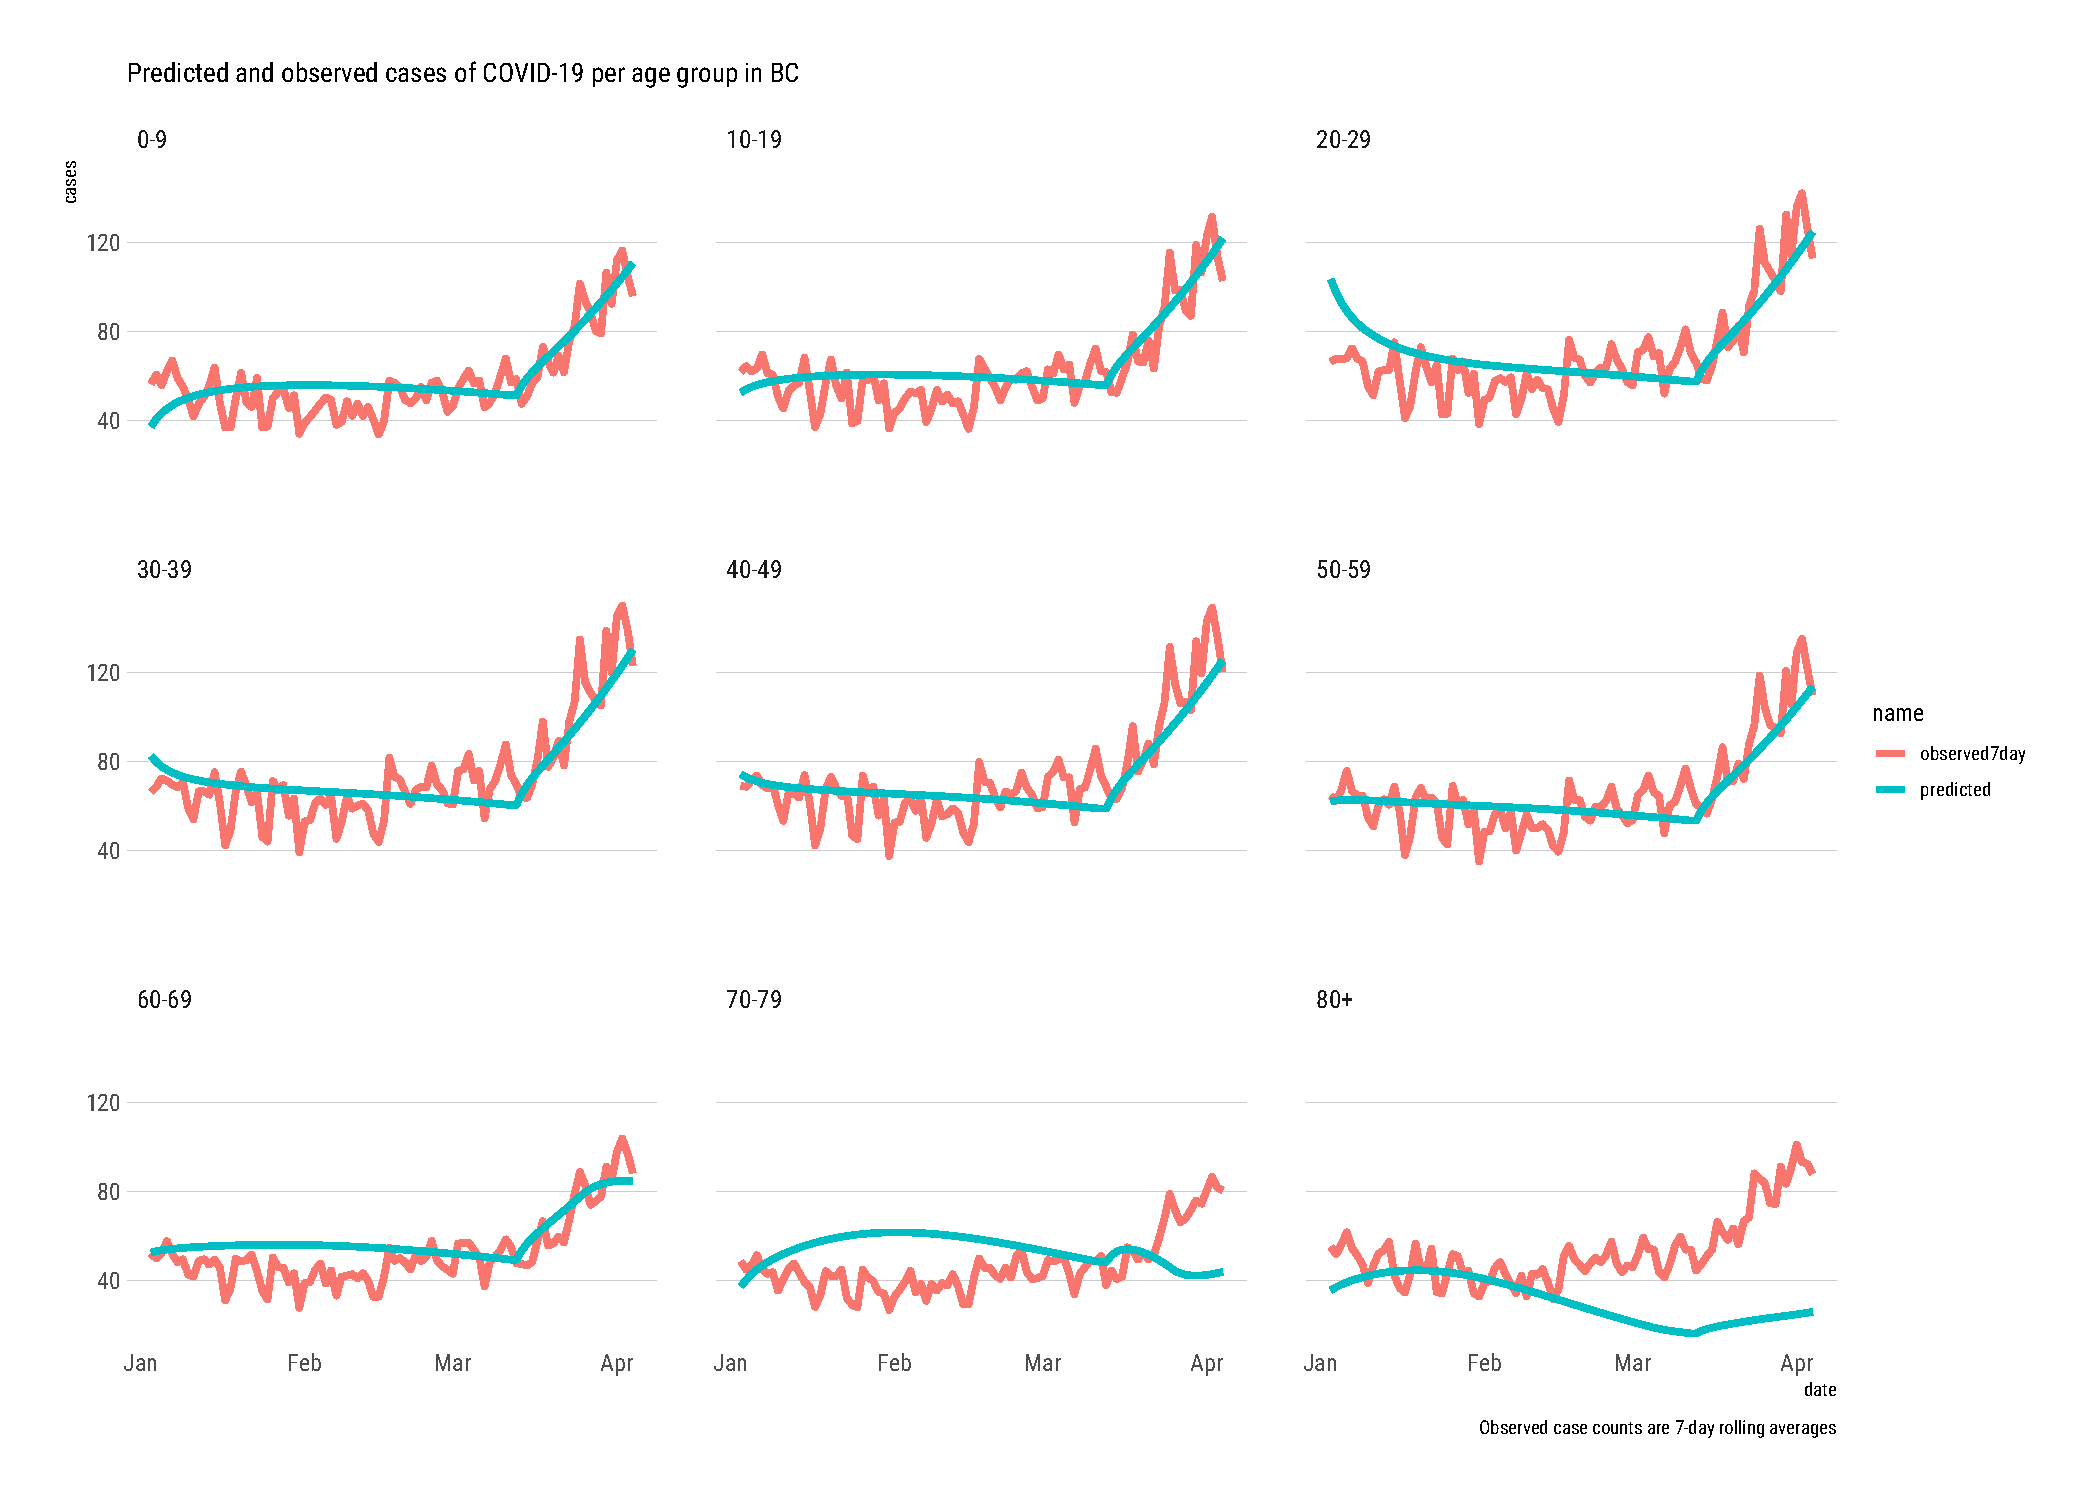
\includegraphics[width=1\linewidth]{../figures/fig-validation} 

}

\caption{Face validity of model case counts}\label{fig:figValidation}
\end{figure}

Predicted epidemiological curve and age-stratified case counts showed
good agreement with observed counts reported by BC CDC, except for the
80 and above age category where the model underestimated case counts
(Figure 1), however, this age group had almost no implications on the
compared scenarios.

\hypertarget{harm-benefit-from-a-societal-perspective}{%
\subsection{Harm-benefit from a societal
perspective}\label{harm-benefit-from-a-societal-perspective}}

EMA evidence as of April 4th, 2021 suggests that if we immediately offer
a first dose of the AZ vaccine to all eligible front-line workers in BC,
the expected number of VIPIT-related deaths by the end of June 2021 is
0.337 {[}95\% CI 0.206-0.498{]}, which means the probability of
observing at least one VIPIT-related death in the same period is 28.6\%.
Adding the risk from the second dose, the expected number of
VIPIT-related deaths until the end of summer is 0.675 {[}95\% CI
0.411-0.987{]}. The probability of observing at least one VIPIT-related
death till the end of the summer will be 49.1\%.

NACI had based its analysis on the PEI estimates of a chance of 1 in
100,000 for VIPIT, and a mortality probability of 40\%, based on the
data that was available in late March. In this worst-case scenario, the
expected number of deaths in BC would be 1 after the first dose is
completed for all front-line workers and 2 after the second doses are
delivered. Details of the calculations can be found in Appendix A.

\begin{figure}

{\centering 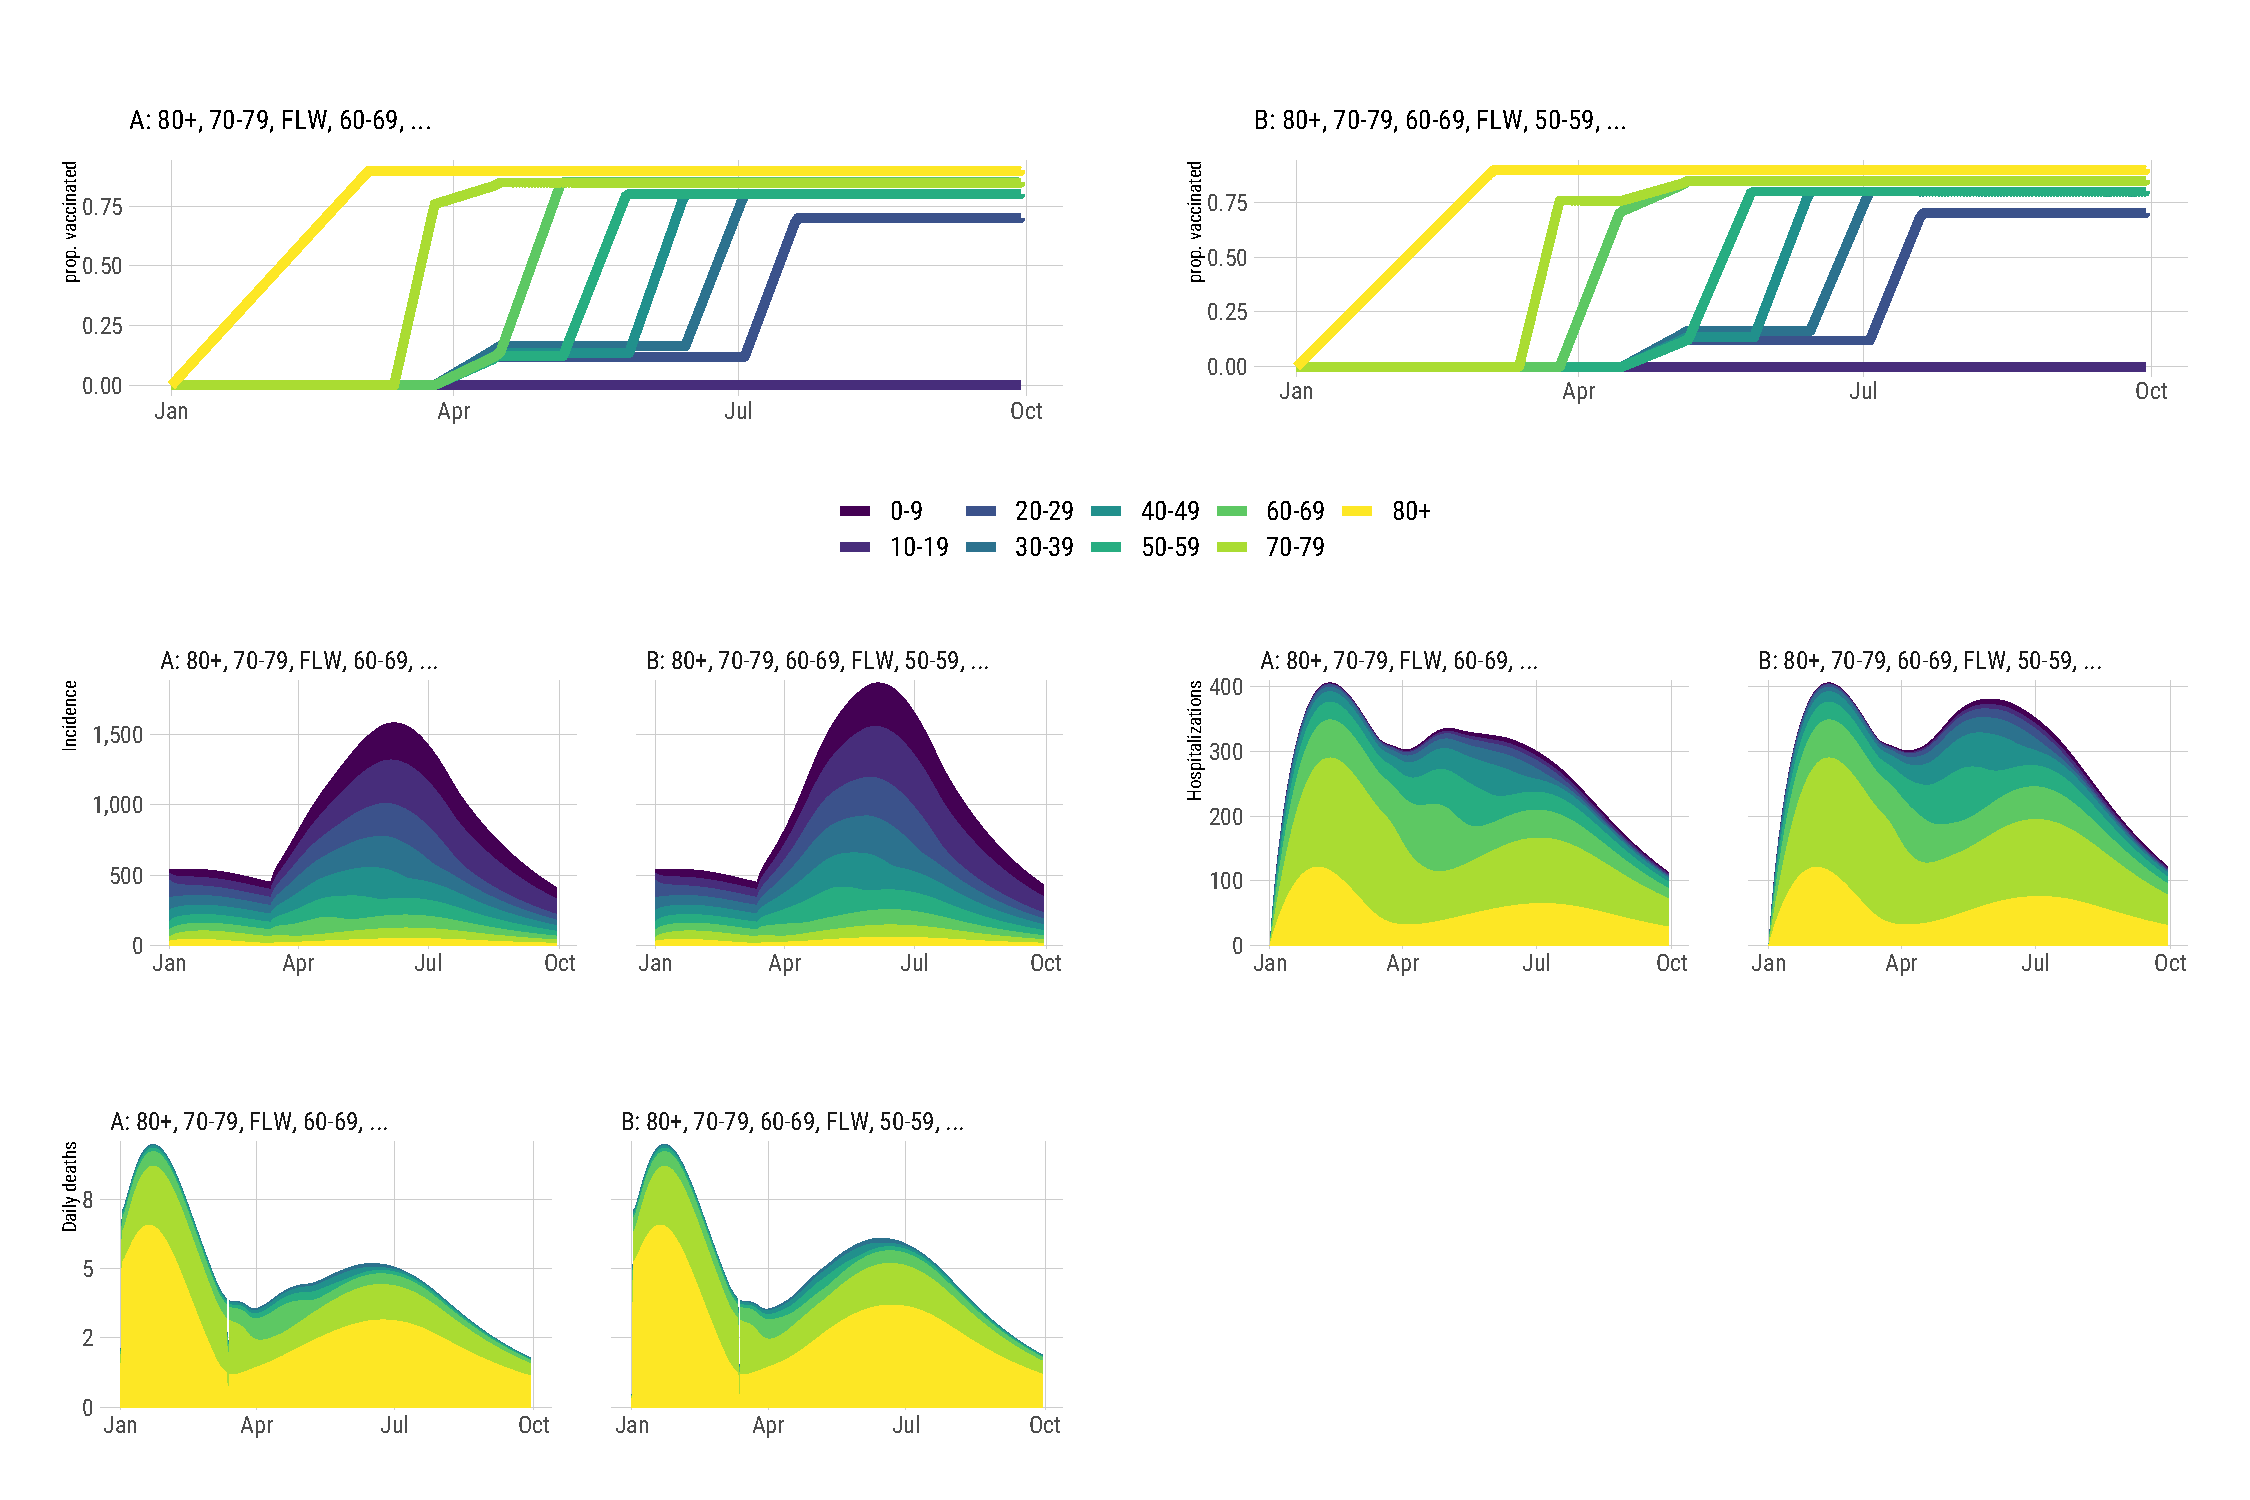
\includegraphics[width=1\linewidth]{../figures/fig-trajectoriesFull} 

}

\caption{Top Panel: Projection of the progression of the vaccination for different age groups and front-line workers (FLW). Bottom Panel: Projection of COVID-19 cases, hospitalizations, and deaths from January 1st to October 1st, 2021.}\label{fig:fig1}
\end{figure}

Figure 2 shows the progression of the vaccination campaign, as well as
projections for COVID-19 cases, hospitalizations, and deaths under the
two scenarios of immediately prioritizing front-line workers (A) and
delaying their vaccination to after all those over 60 years of age are
offered a dose of the vaccine and then offer them an mRNA vaccine (B).

In our analysis, Scenario A led to 27175 fewer cases of COVID-19, 506
fewer hospitalizations, 87 fewer deaths, and 1462 fewer cases of Long
COVID, assuming \(R_0=1.35\). Appendix B includes results of the
sensitivity analysis for a wider range of values for \(R_0\) and the
effectiveness of the vaccine against transmission, \(v_e\).

\hypertarget{harm-benefit-from-an-individual-risk-perspective}{%
\subsection{Harm-benefit from an individual risk
perspective}\label{harm-benefit-from-an-individual-risk-perspective}}

\begin{figure}

{\centering 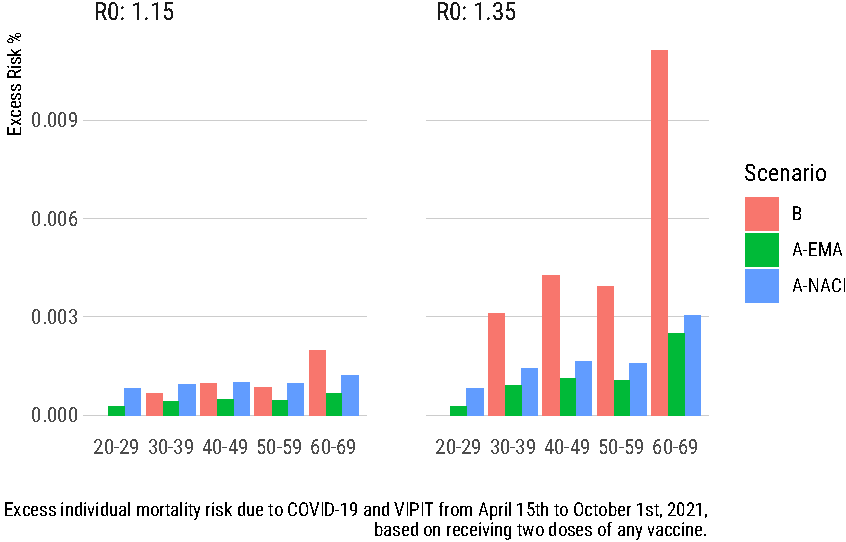
\includegraphics[width=0.9\linewidth]{theCaseforAZ_files/figure-latex/covidvsvipit-1} 

}

\caption{ Comparison of excess mortality risk for different age groups based on the COVID-19 risk caused by delayed vaccination (B) and estimated residual COVID-19 and VIPIT risk (A) by the EMA and NACI}\label{fig:covidvsvipit}
\end{figure}

Figure 3 compares the risk of VIPIT-related mortality from 2 doses of
the AZ vaccine and residual risk from COVID-19, with the mortality risk
from COVID-19 due to delayed vaccination from April 1st to October 1st,
2021. We did the comparison under two scenarios of an \(R_0\) of 1.15 or
1.35, to represent different intensities for the third wave, or
alternatively to represent different geographical parts of the province
during the third wave. We calculated the mortality risk associated with
VIPIT using both the latest and most comprehensive evidence by EMA, and
the worst-case scenario using the evidence considered by NACI. Using EMA
estimates, we found that under both \(R_0\) scenarios, the mortality
risk due to COVID-19 to be much higher than the mortality risk
associated with VIPIT in those over 40. Mortality risk from COVID-19 was
also higher than that of VIPIT for the 30-39 age group, although the
difference was negligible under \(R_0\) of 1.15 scenario. For the 20-29
age group, the estimated mortality risk of vaccination with the AZ
vaccine was higher than that of COVID-19. Using the worst-case VIPIT
estimates considered by NACI, mortality risk from COVID-19 was
considerably higher than that of VIPIT for those over 60 in all areas
and those over 30 in high-risk areas (\(R_0=1.35\)).

\hypertarget{discussion}{%
\section{Discussion}\label{discussion}}

In its analysis of AZ vaccine published on March 29th, 2021, NACI
weighed the risk of adverse events against the age-stratified risk of
mortality due to COVID-19, and concluded that the AZ vaccine should not
be used in adults under 55 years of age pending an overall
risk-assessment. Our analysis confirms that given the evidence available
in late March (a risk of 1 in 100,000 for VIPIT and a 40\% case
fatality) and the lower rates of transmission (i.e.~a lower \(R_0\)) at
that time, suspending the use of AZ vaccine in younger adults would have
been advisable. However, as of April 8th, 2021, the evidence has evolved
and the EMA is now reporting a risk of 1 in 153,000 for VIPIT and a 20\%
case fatality. These latest estimates together with a new wave of the
disease have changed the harm-benefit landscape considerably. In
addition, the benefits of the AZ vaccine go beyond preventing
COVID-related mortality and include protection against other possible
COVID-19 complications in younger adults including hospitalizations and
associated risk of venous thromboembolism (VTE; Rates are about 2 folds
higher in hospitalized COVID-19 patients than that of medical
non-COVID-19 inpatients \citep{alberta_health_services_covid-19_2021}),
and Long COVID, as well as preventing onward transmission of the virus,
as evident in the recent sharp decline of COVID-19 cases in the UK
\citep{govuk_official_2021}.

The UK vaccination program started on December 8th with the
Pfizer-BioNTech vaccine and was complemented with the AZ vaccine since
January 4th. The number of confirmed daily COVID-19 cases in the UK has
plummeted from about 60,000 cases a day in early January 2021 when a
national lockdown was imposed and about 3\% of the population had
received at least one vaccine dose, to about 11,000 cases per day on
February 22, 2021 when a roadmap to easing the lockdown was announced,
to about 6000 cases per day on March 8, 2021 when the first phase of
easing public health restrictions was commenced
\citep{bbc_lockdown_2021} and has continuously declined since then to
just above 2589 cases as of April 10th, 2021, when 61\% of the UK
population had received one dose of a COVID-19 vaccine
\citep{govuk_official_2021}.

In addition to the death aversion resulting from strict public health
measures, based on a recent analysis by Public Health England and the
University of Warwick, it has been estimated that as of March 31, 2021,
10,400 deaths have been avoided in the UK solely due to the direct
implementation of a nationwide vaccination program (indirect effects
were not measured; 87.5\% of these averted deaths were in the 80+ years
old age group, 11.5\% of them in 70-79, and 1\% in 60-69 years old age
group) \citep{public_health_england_impact_2021}. As about half of all
vaccine doses administered in the UK have been AZ vaccines, and based on
the estimated AZ vaccine efficacy of about 76\% against symptomatic
COVID-19 and 64\% against any NAAT-positive COVID-19 infection between
22 and 90 days after the first dose \citep{voysey_single-dose_2021}, and
real-world single-dose AZ vaccine effectiveness of about 60\% against
symptomatic COVID-19 and 80\% against COVID-19 hospitalization
\citep{public_health_england_1public_2021}, it is clear that the AZ
vaccine is effective in reducing the overall burden of COVID-19.

Potential prevention of onward transmission with the AZ vaccine could be
especially critical for front-line workers during the current wave of
COVID cases. Of note, two recent studies from Toronto, Ontario have
shown that neighbourhoods with the highest proportion of front-line
workers had per capita COVID-19 case and death rates that were 2.5-3
folds higher than that of neighbourhoods with the lowest share of
front-line workers
\citep[\citet{rao_disproportionate_2021}]{chagla_characterizing_2021}.

Based on our analysis, immediately making the AZ vaccine available to
front-line workers is, assuming optimal uptake, net-beneficial by a wide
margin from a societal perspective. Our analysis from an individual risk
perspective shows that the risk of contracting COVID-19 and dying from
it due to delayed vaccination is considerably higher than the risk of
dying from VIPIT in those over 40, and also in those over 30 in
high-risk areas.

For a public health intervention to be deemed ethically acceptable,
being net-beneficial at a societal level is not enough in and of itself.
Not all interventions that are net-beneficial at a societal level are
net-beneficial for each member of the society, as those who carry the
burden of the risk of adverse events may not be the same people who reap
the benefits. We also recognize that many might intuitively consider
mortality due a public health intervention in an otherwise healthy
person to be ethically worse than failing to protect someone from
mortality due to COVID-19. While we are not going to solve the trolley
problem here, we believe that our conclusions hold regardless of the
position we take with respect to the \emph{doing vs.~allowing harm}
problem \citep{woollard_doing_2016}, as long as the expected benefits
outweigh the risk at a personal level, as seems to be the case for most
age groups in our study.

Our analysis was based on the assumption that immediate deployment of
alternative mRNA vaccines for front-line workers was not logistically
feasible. If feasible, offering mRNA vaccines to front-line workers will
be more in line with the principle of reciprocity outlined in the BC
COVID-19 Ethical Decision-Making Framework \citep{bccdc_covid-19_2020},
and the more general principle of justice in bioethics
\citep{mccormick_principles_2021}, based on the fact that as of April
10th, 2021, no VIPIT cases have been linked to COVID-19 mRNA vaccines.
From a vaccine efficacy point of view, determining the
\emph{superiority} of one vaccine to the other is not straightforward;
there is more to the apparent but variable 5\%-33\% efficacy gap
(symptomatic COVID-19; 7-14 days after second dose) between mRNA and AZ
COVID-19 vaccines
\citep{polack_safety_2020, baden_efficacy_2021, astrazeneca_azd1222_2021, emary_efficacy_2021}
than meets the eye, including differences in study populations,
settings, time periods, and vaccine storage requirements
\citep{ledford_why_2021}. Importantly, these vaccines were comparable in
efficacy against severe COVID-19 in phase 3 trials
\citep{abdool_karim_new_2021, astrazeneca_azd1222_2021}. Considering
emerging real-world vaccine effectiveness data, two studies in the UK
demonstrated that one dose of the Pfizer-BioNTech mRNA vaccine or the AZ
vaccine have a comparable performance in terms of reducing rates of
PCR-positive SARS-CoV-2 infection, symptomatic COVID-19, and
COVID-19-related hospitalizations
\citep{shrotri_vaccine_2021, jamie_lopez_bernal_early_2021}.

Our findings are corroborated by the the recent recommendation of the UK
Joint Committee on Vaccination and Immunisation (JCVI) that the benefits
of the AZ vaccine far outweigh the risk in 30 years old or older
recipients \citep{jcvi_jcvi_2021}.

\hypertarget{limitations}{%
\section{Limitations}\label{limitations}}

Our analysis from an individual risk perspective was based on average
rates of COVID-19 and its related outcomes per age group. However, the
true risk within age groups is still heterogeneous and is affected by
many factors including but not limited to exposure, medical history,
work environment, and socioeconomic status.

Our analysis did not consider social aspects of vaccine roll-out such as
the effect of different roll-out strategies on uptake and vaccine
hesitancy, as they were beyond our expertise. However, we recognize that
each time a recommendation for vaccine safety is reversed, there might
be a penalty in public trust which could fuel vaccine hesitancy.
Potential for these effects should be weighed carefully by policy
makers.

Our analysis is based on currently available estimated rates of 1 in
million to 1 in 100,000 for VIPIT and might need correction should
higher rates of this complication be reported.

We have not considered potential sex differences in the risk for VIPIT.
Although cases identified to date have been predominantly female, it
remains unclear whether this was due to more females receiving the AZ
vaccine or due to an intrinsic difference in risk.

\hypertarget{conclusions}{%
\section{Conclusions}\label{conclusions}}

Current evidence suggests that benefits of immediate prioritization of
front-line workers for vaccination with the AZ vaccine far outweigh the
risk, both at a societal and at a personal level for those over 40 years
of age, and those over 30 years of age in high-risk areas. Ultimately,
in dynamic situations like this where the evidence is uncertain and
evolving, vaccine roll-out decisions are judgment calls that need to
take a complex network of medical, epidemiological, ethical, logistics,
and societal considerations into account.

\bibliographystyle{tfcad}
\bibliography{AZVIPIT.bib}


\input{"appendix.tex"}


\end{document}
